\chapter{Metody evaluace}\label{cha:evaluace}

V této sekci prezentujeme zavedené a standardní způsoby vzájemného kvantitativního i kvalitativního porovnávání výsledků metod pro extrakci melodie, které vychází z postupů evaluace v soutěži MIREX. V první sekci uvádíme soutěž MIREX jako takovou, následně definujeme používané metriky a v závěru kapitoly zmiňujeme některé praktické metriky používané při trénování modelů v této práci.

\section{MIREX}

Soutěž MIREX (Music Information Retrieval Evaluation eXchange) probíhá již od roku 2005 a v MIR komunitě zastává hlavní postavení jakožto každoroční událost pro nezávislé, objektivní srovnání state-of-the-art metod a algoritmů pro řešení širokého spektra úloh souvisejících se zpracováním hudebních dat. Mezi tyto úlohy patří například rozpoznání žánru, odhad tempa, odhad akordů, identifikace coveru a samozřejmě také extrakce melodie.

Na rozdíl od jiných úloh, kde debata o zvolení nejvhodnějších objektivních metrik pro porovnávání metod stále probíhá, metriky pro extrakci melodie se ustanovily již v prvním ročníku (na základě dřívějších zkušeností) a zůstaly neměnné dodnes \citep{Raffel2014}. Naopak data použitá pro testování se postupně kumulují a dnes soutěž probíhá již s řadou datasetů (ADC04, MIREX05, MIREX08, MIREX09, ORCHSET15). V tabulce \ref{tab:mirex_datasety} uvádíme přehled těchto evaluačních datasetů.

\subsection{Formát výstupu v soutěži MIREX}

Obvyklý formát výstupu algoritmů je CSV soubor se dvěma sloupci. První sloupec obsahuje pravidelné časové značky, standardně délky $10\,\rm ms$, případně $\frac{256}{44\,100} \doteq 5.8 \,\rm ms$. Druhý sloupec pak odhad základní frekvence melodie. Nepřítomnost melodie se označuje hodnotou frekvence 0. Některé algoritmy uvádí i odhady výšky základní frekvence mimo detekovanou melodii (může jít například o doprovod, který zní i po hlavním melodickém hlasu). Aby tyto odhady byly odlišené od odhadů hlavní melodie, jsou uvedeny v záporných hodnotách. Díky tomu pak lze nezávisle vyhodnotit přesnost \textit{odhadu výšky} a \textit{detekce melodie}. Odhad výšky se vyhodnocuje podle absolutní hodnoty frekvence ve všech časových oknech, ke kterým existuje anotace, detekce melodie pak na všech hodnotách vyšších než 0. 

Formát CSV pro zápis anotací melodie, který byl zaveden v rámci soutěže MIREX, dodržují také všechny dostupné datasety a ačkoli existují pokusy o změnu tohoto formátu \citep{Humphrey2014a}, MIREX formát je natolik jednoduchý a prozatím dostačující, že k přechodu na sofistikovanější formáty zatím nedošlo. Pro ilustraci přikládáme část referenční anotace ženského zpěvu, v anotaci se vyskytuje krátká pomlka mezi znějícími tóny. Grafické znázornění referenční anotace melodie celé nahrávky můžeme nalézt v úvodu na obrázku \ref{obr:input_output}.

%$
\begin{code}[xrightmargin=20em]

8.568     381.349
8.574     379.959
8.580     378.229
8.586     376.067
8.591     372.236
8.597     369.793
8.603     0.000
8.609     0.000
8.615     0.000
8.620     0.000
8.626     0.000
8.632     0.000
8.638     352.272
8.644     338.922

\end{code}
%$

\begin{table}[h!]
\centering
\begin{tabular}{p{2.5cm}p{11cm}}
\toprule
Dataset        & Popis \\
\midrule
ADC2004        & 20 výňatků délky kolem 20 sekund, žánry pop, jazz, opera. Obsahuje živé a syntetické MIDI nahrávky. Celková délka 369 sekund. Dataset je kompletně zveřejněn. \\
MIREX05        & 25 výňatků délky 10-40 sekund, žánry rock, R\&B, pop, jazz a sólové piano. Obsahuje živé a syntetické MIDI nahrávky. Celková délka 686 sekund. K datasetu je dostupná trénovací množina MIREX05train \\
INDIAN08       & Čtyři minutové výňatky tradičního zpěvu z oblasti severní Indie. Ke každému výňatku existují dvě verze s různě hlasitým doprovodem, celkově se tedy dataset skládá z osmi nahrávek. Celková délka 501 sekund. Dataset je neveřejný \\
MIREX09 ($0\,\rm dB$)  & 374 čínských karaoke písní. Poměr hlasitosti zpěvu k doprovodu je 0dB. Celková délka $10\,020$ sekund. K datasetu je dostupná trénovací množina MIR1K \\
MIREX09 ($-5\,\rm dB$) & Stejné výňatky jako v případě MIREX09 ($0\,\rm dB$), poměr hlasitosti zpěvu k doprovodu je však -5dB. Celková délka $10\,020$ sekund. \\
MIREX09 ($+5\,\rm dB$) & Stejné výňatky jako v případě MIREX09 ($0\,\rm dB$), poměr hlasitosti zpěvu k doprovodu je však +5dB. Celková délka $10\,020$ sekund. \\
ORCHSET15      & 64 orchestrálních výňatků z různých období vývoje klasické hudby. Anotace melodie je uvedena s přesností jednoho půltónu, Celková délka 1404 sekund. Dataset je kompletně zveřejněn. \\
\bottomrule
\end{tabular}
\caption{Přehled evaluačních datasetů v soutěži MIREX, částečně převzato z práce \cite{Salamon2014}.}\label{tab:mirex_datasety}
\end{table}

\section{Trénovací, validační a testovací množina}

Z dostupných dat, které pro úlohu máme k dispozici, musíme vyhradit množiny pro trénování, validaci a testování, aby byly metody porovnatelné jak mezi sebou, tak se stávajícími state-of-the-art metodami. Pro trénování se jeví jako nejvhodnější dataset MedleyDB, jednak pro svou délku a jednak pro žánrovou rozmanitost, proto je použit pro všechny popsané experimenty. Rozdělení datasetu na trénovací, validační a testovací množiny jsme převzali z práce \cite{Bittner2017}, díky tomu je korektní naše výsledky na testovací množině MedleyDB přímo porovnávat s výsledky uvedenými v článku. Tento postup využití existujícího rozdělení dat používá ve své práci také \cite{DBasaranSEssid2018}, i s jeho výsledky proto naši práci můžeme porovnávat.

Data byla rozdělena na trénovací, validační a testovací množinu tak, aby skladby od jednoho interpreta náležely právě do jedné z množin. Využili jsme existujícího rozdělení používaného v článcích \cite{Bittner2017} a \cite{DBasaranSEssid2018}, validační i testovací výsledky jsou tedy díky tomu porovnatelné s výsledky uvedenými v článcích.

% Další výhodou použití stejného \textit{splitu} je možnost replikace výsledků, za použití popisované architektury, a tím pádem minimalizování možnosti nějaké velké implementační chyby v kódu. Pokud by se totiž výsledky nepodařilo replikovat se stejnými daty i architekturou, musela by být chyba jinde - tedy s největší určitostí v vyvinutém frameworku.

Dalším užitečným zdrojem dat je dataset MDB-melody-synth, který je syntetizován z vícestopých nahrávek MedleyDB. Proto je vhodné použít stejné rozdělení dat, jaké se používá pro MedleyDB, protože data budou silně korelovaná s původními nahrávkami a tak bychom mohli dojít k chybným, uměle vysokým výsledkům, pokud bychom množiny změnili. Jelikož dataset neobsahuje veškerá data, ale pouze jejich podmnožinu, i v experimentech používané rozdělení dat obsahuje pouze podmnožinu z původního rozdělení datasetu MedleyDB. 

Posledním velkým datasetem používaným v práci, je Weimar Jazz Database. Původním záměrem bylo dataset použít i pro trénování a validaci metod proto jsme jej rozdělili na datové množiny, nakonec byla však použita pouze testovací množina. Při rozdělování datasetu jsme postupovali podle práce \cite{Bittner2017}, data jsme rozdělili na tři části. Skladby jsou rozděleny do částí podle interpretů tak, aby se každý interpret vyskytoval právě v jedné části datasetu. Toto omezení na podmnožiny \cite{Bittner2017} nediskutuje, lze však doložit (práce \cite{Sturm2013}), že pro úlohu rozpoznání žánru metody založené na strojovém učení vykazují po trénování a validaci na datech bez tohoto filtru výrazně lepší výsledky než stejné metody spuštěné na roztříděných datech, takové zlepšení výkonu je ale jistě umělým důsledkem špatné volby trénovací množiny. 

Délky a počty nahrávek datových množin používaných v této práci shrnujeme v tabulce \ref{tab:data_splits}, přesný výčet skladeb použitých v každé množině je v příloze práce.

\begin{table}[h!]
\centering
\begin{tabular}{llll}
\toprule
Dataset          & Množina & Počet nahrávek & Délka \\
\midrule
MedleyDB         & train   & 67             & $3.06\,\rm h$ \\
                 & valid   & 15             & $0.85\,\rm h$ \\
                 & test    & 27             & $1.71\,\rm h$ \\
MDB-melody-synth & train   & 44             & $1.88\,\rm h$ \\
                 & valid   & 8              & $0.46\,\rm h$ \\
                 & test    & 14             & $0.87\,\rm h$ \\
WJazzD           & train   & 169            & $5.49\,\rm h$ \\
                 & valid   & 54             & $1.25\,\rm h$ \\
                 & test    & 74             & $2.08\,\rm h$ \\
\bottomrule
\end{tabular}
\caption{Přehled trénovacích, validačních a testovacích množin použitých v práci.}\label{tab:data_splits}
\end{table}

Dále k testování používáme datasety ADC04, MIREX05train a ORCHSET, blíže popsané v kapitole \nameref{cha:datasety}. Protože jsou datasety ADC04 a ORCHSET jsou v práci použity pouze jako testovací data, můžeme výsledky přímo srovnávat s odpovídajícími žebříčky úlohy Melody Extraction v soutěži MIREX.

% ------

% - MatthewEntwistle_FairerHopes
% obsahuje harfu, ale trénovací data ji neobsahují, chce to ale víc prozkoumat, jelikož trénovací data neobsahují víc nástrojů, tak zjistit přesně přesnost anotace pro tyto nástroje


\section{Metriky}

Celková kvalita výstupu metody pro extrakci melodie je určena její schopností odhadnout správně výšku tónu hrající melodie a také rozpoznat části skladby, které melodii neobsahují. Jelikož jsou tyto podúlohy na sobě nezávislé, standardní sada metrik zahrnuje jak celkové vyhodnocení přesnosti, tak dílčí vyhodnocení pro \textit{odhad výšky} a \textit{detekci melodie}. 

V práci pracujeme s metrikami vypočítanými na validačních a testovacích sadách, ty se počítají jako průměr výsledků na jednotlivých skladbách v sadě.

% -------

% - můžu zmínit to, že je toto rozdělení důležité pro Orchset, který je z většiny voiced, a tedy overall accuracy může být zavádějící u algoritmů s přísným voicing detection.
% - celkové skóre na datasetu je průměr všech písní


\subsection{Definice metrik}

Většina metrik je definována na základě porovnávání jednotlivých anotačních oken --- tedy typicky srovnáním odhadovaných a pravdivých výšek melodie po konstantních časových skocích. Datasety používané pro vyhodnocování v soutěži MIREX používají časový skok délky 10 ms. V definicích budu vycházet ze značení v práci \cite{Salamon2014}. 

    Označme vektor odhadovaných základních frekvencí $\mathbf{f}$ a cílový vektor $\mathbf{f^*}$, složka $f_\tau$ je buď rovna hodnotě $f_0$ melodie, nebo $0$, pokud v daném čase melodie nezní. Obdobně zaveďme vektor indikátorů $\mathbf{v}$, jehož prvek na pozici $\tau$ je roven $v_\tau=1$, pokud je v daném časovém okamžiku detekována melodie a $v_\tau = 0$ v opačném případě. Podobným způsobem zavedeme i vektor cílových indikátorů melodického hlasu $\mathbf{v^*}$ a také vektor indikátorů absence melodie $\bar{v}_\tau = 1 - v_\tau$. 

\begin{figure}[h!]\centering
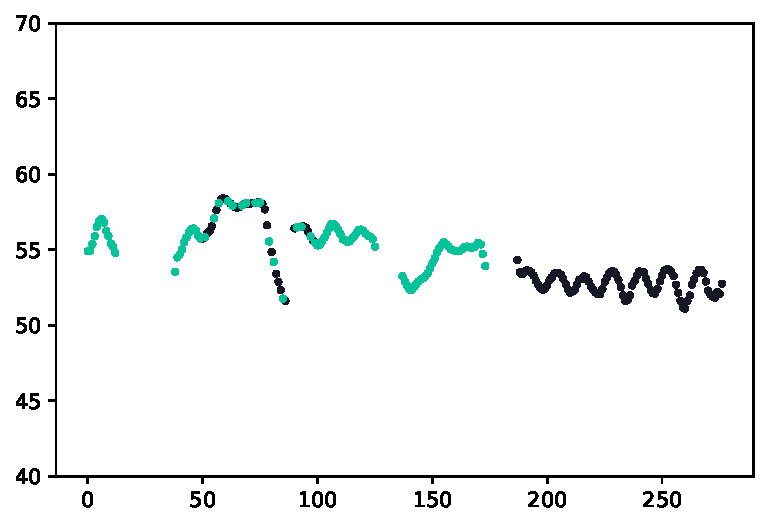
\includegraphics[scale=0.5]{../img/chyba_VR}
\caption{Příklady chyb špatné detekce melodie negativně ovlivňující metriku VR.}
\label{obr:chyba_VR}
\end{figure}

\subsubsection{Voicing Recall rate (Úplnost detekce)}

Poměr počtu časových oken, které byly správně označené jakožto obsahující melodii, a počtu časových oken doopravdy obsahujících melodii podle anotace.

    $$\mathrm{VR}(\mathbf{v}, \mathbf{v^*}) = \frac{\sum_\tau{v_\tau v^*_\tau}}{\sum_\tau{v^*_\tau}}$$

\begin{figure}[h!]\centering
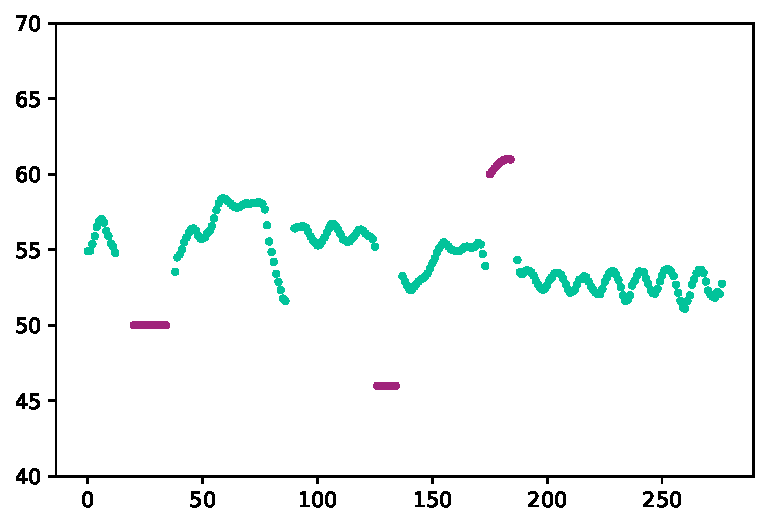
\includegraphics[scale=0.5]{../img/chyba_VFA}
\caption{Příklady chyb špatné detekce melodie zvyšující metriku VFA.}
\label{obr:chyba_VFA}
\end{figure}

\subsubsection{Voicing False Alarm rate (Nesprávné detekce)}

Poměr počtu časových oken, které byly nesprávně označené jako obsahující melodii, a počtu časových oken, které doopravdy melodii neobsahují. Pro interpretaci této metriky platí, že nižší hodnota je lepší, vyšší hodnota je horší.

    $$\mathrm{FA}(\mathbf{v}, \mathbf{v^*}) = \frac{\sum_\tau{v_\tau \bar{v}^*_\tau}}{\sum_\tau{\bar{v}^*_\tau}}$$


\begin{figure}[h!]\centering
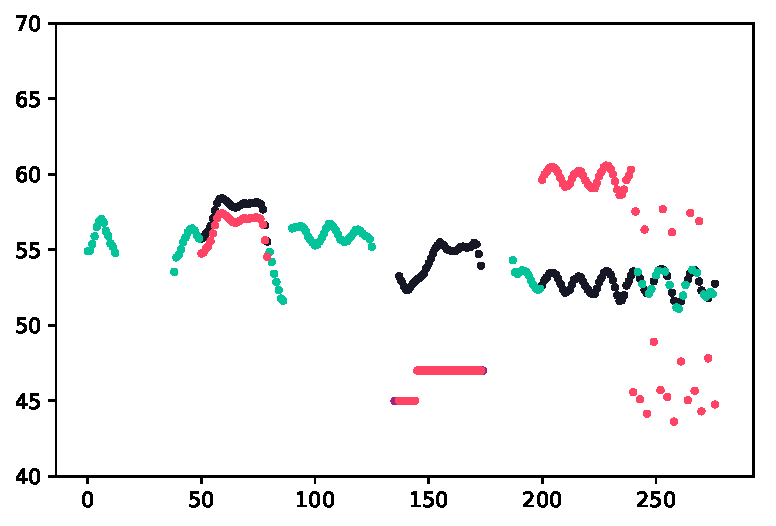
\includegraphics[scale=0.5]{../img/chyba_RPA}
\caption{Příklady chyb ovlivňujících metriku RPA a RCA.}
\label{obr:chyba_RPA}
\end{figure}


\subsubsection{Raw Pitch Accuracy (Přesnost odhadu výšky)}

Poměr správně odhadnutých tónů k celkovému počtu oken, které obsahují melodii. Výška správně určeného tónu se může lišit až o jeden půltón.


    $$\mathrm{RPA}(\mathbf{f}, \mathbf{f^*}) = \frac{\sum_\tau{v^*_\tau v_\tau \mathcal{T}[\mathcal{M}(f_\tau) - \mathcal{M}(f^*_\tau)}] }{\sum_\tau{v^*_\tau}}$$

kde $\mathcal{T}$ je prahová funkce

    \begin{equation*}
        \mathcal{T}[a] = \begin{cases}
                1 & \mathrm{pro} \abs{a} \le 0.5 \\
                0 & \text{jinak}
                
            \end{cases}
    \end{equation*}

Dodáme, že práh $0.5$ je v některých případech použití vhodné snížit na restriktivnější hodnoty, jako je $0.25$ nebo dokonce $0.1$. Jedná se zejména o použití metriky pro úlohu odhadu výšky jednohlasu (jako například v práci \cite{Kim2018}).

a $\mathcal{M}$ je funkce zobrazující frekvenci $f$ na reálné číslo počtu půltónů od nějakého referenčního tónu $f_{\mathrm{ref}}$ (například od 440 Hz, tedy komorního A4).

    $$\mathcal{M}(f) = 12 \log_2(\frac{f}{f_{\mathrm{ref}}})$$


\begin{figure}[h!]\centering
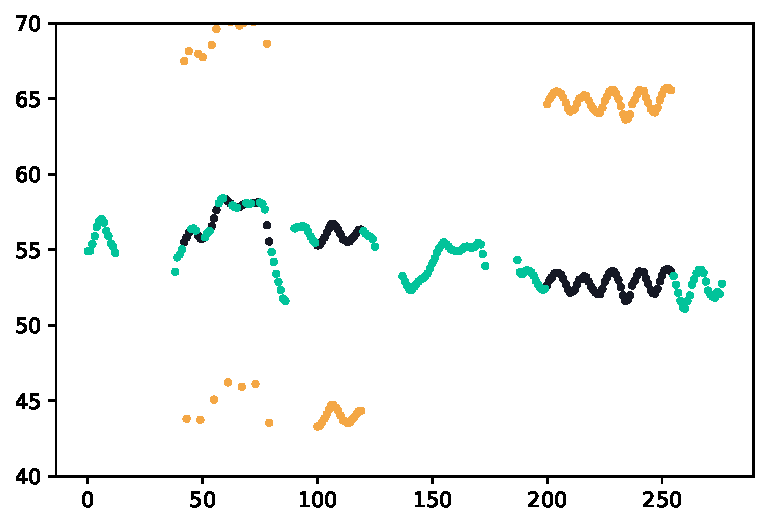
\includegraphics[scale=0.5]{../img/chyba_RCA}
\caption{Příklady chyb \uv{o oktávu} ovlivňujících pouze metriku RPA, nikoli metriku RCA.}
\label{obr:chyba_RPA}
\end{figure}

\subsubsection{Raw Chroma Accuracy (Přesnost odhadu výšky nezávisle na oktávě)}

Počítá se podobně jako \textit{Přesnost odhadu tónu}, výstupní a cílové tóny jsou však mapovány na společnou oktávu. Metrika tedy ignoruje chyby odhadu způsobené špatným určením oktávy tónu.

    $$\mathrm{RCA}(\mathbf{f}, \mathbf{f^*}) = \frac{\sum_\tau{v^*_\tau v_\tau \mathcal{T}[\langle \mathcal{M}(f_\tau) - \mathcal{M}(f^*_\tau)} \rangle_{12}] }{\sum_\tau{v^*_\tau}}$$

Nezávislost na oktávě zajistíme pomocí zobrazení rozdílu cílového a výstupního tónu na společnou oktávu.

    $$\langle a \rangle_{12} = a - 12 \lfloor \frac{a}{12} + 0.5 \rfloor  $$


\subsubsection{Overall Accuracy (Celková přesnost)}

Celková přesnost měří výkon algoritmu jak v odhadu melodie tak v detekci melodie. Počítá se jako podíl správně odhadnutých oken a celkového počtu oken.

    $$\mathrm{OA}(\mathbf{f}, \mathbf{f^*}) = \frac{\sum_\tau{v^*_\tau v_\tau \mathcal{T}[\mathcal{M}(f_\tau) - \mathcal{M}(f^*_\tau)}] + \bar{v}^*_\tau \bar{v}_\tau }{L}$$

\subsubsection{Poznámka k definicím metrik}

Definice RPA, RCA a OA zde uvedené se mírně liší od výchozích v práci \cite{Salamon2014}, jejich přímá implementace podle vzorce totiž vede kvůli nedostatečně dobře zadefinovanému vektoru frekvencí $\mathbf{f}$ k chybě, která se týká zejména metriky RCA. Ta v původním znění definice chybně zahrnovala jako správné tóny ty, které algoritmus odhadl jako nulové (tedy neznějící) a zároveň jejich pravdivá hodnota byla po zobrazení na jednu společnou oktávu blízká nule (tedy původní tón byl blízký nějakému násobku referenční frekvence). Kvůli zobrazení na společnou oktávu se stanou \uv{neznělé nulové odhady} a tóny blízké referenčním frekvencím nerozlišitelné a byly nesprávně považované za korektní. \footnote{
    Tato chyba byla přítomná i v nejpoužívanější, veřejné implementaci MIR metrik \textit{mir\_eval}. V praxi rozdíl chybné a opravené hodnoty této metriky na datasetu MedleyDB mohla dosahovat až sedmi procentních bodů, na repozitáři hostovaném na serveru Github jsme již spolu s autory chybu odstranili (odkaz na Github issue: \url{https://github.com/craffel/mir_eval/issues/311}). Opravný patch bude zahrnut do další verze balíku. Výsledky v této práci jsou počítány s opravenou verzí.}

\subsection{Další metriky}

Protože princip vnitřního fungování neuronových sítí často není zřejmý, je užitečné mít co nejvíce různých indikátorů, abychom měli při porovnávání jednotlivých modelů alespoň podrobnou informaci, v jakých ohledech se síť zlepšuje nebo zhoršuje. Pro tento účel jsem při práci implementoval další metriky, které při hledání architektur sítí pomáhaly.

\subsubsection{Chroma Overall Accuracy}

Počítá se obdobně jako Overall Accuracy, ale tóny jsou mapovány na společnou oktávu.

\subsubsection{Raw Harmonic Accuracy}

Metrika počítá odhadovaný tón jako správný, pokud se trefil do některé z harmonických frekvencí tónu. Protože je harmonických frekvencí teoreticky nekonečné množství, parametrem metriky je do jakého celočíselného násobku se ještě odhad počítá.

    $$\mathrm{RHA}(\mathbf{f}, \mathbf{f^*}, n) = \frac{\sum_{k=1}^n \sum_\tau{v^*_\tau v_\tau \mathcal{T}[\mathcal{M}(f_\tau) - \mathcal{M}(k f^*_\tau)} ] }{\sum_\tau{v^*_\tau}}$$

\subsubsection{Matice záměn not}

Pro podrobnější souhrnný přehled četností chyb se pro klasifikační úlohy používá matice záměn. Sloupce označují správné noty, řádky odhadované. Buňka na pozici $(x,y)$ má pak hodnotu podle četnosti odhadu noty $y$ místo správné noty $x$.

\subsubsection{Histogram vzdáleností odhadu}

Histogram hodnot rozdílu $\mathcal{M}(\mathbf{f}) - \mathcal{M}(\mathbf{f^*})$, tedy histogram vzdáleností odhadů výšky tónů od správné hodnoty.


\subsubsection{Kvalitativní příklady}

Modely byly při práci vyhodnocovány na několikaminutových množinách výňatků z validačních a testovacích dat. Metodika výběru spočívala v poslechu nahrávek a ručním výběru zajímavých hudebních jevů. Několik ukázek bylo také vybráno na základě seřazení nahrávek podle úspěšnosti přepisu stávajícími metodami a výběrem výňatků z tohoto seznamu nejproblematičtějších příkladů.



% - confusion matrix
% - estimation distance histogram
% - pitch accuracy per note

% \subsection{Limitace základních metrik}
% - limitace jsou předvedeny v onsets+frames
%     - nakonec nejsou, tam kritizují jenom 
% - například je otázka, jestli jsou všechny framy stejně důležité - zejména u vybrnkávání, piana, perkusí je otázka, kdy ještě anotovat, tedy jsou tam sporné konce. Na small_valid je to hodně vidět na té harfě
% - nijak se nepenalizuje nekontinualita výstupů, je rozdíl mezi 50\% accuracy, kde je zbytek unvoiced a 50\% accuracy, kde odhady strašně skáčou

% - Bosch metrics \cite{Bosch2016}
%     - Weighted Raw Chroma accuracy - počítá vzdálenost v oktávách
%     - Octave Jumps - vyjadřuje skokovitost o oktávy v po sobě následujících framech v rámci správných chroma odhadů
%     - Chroma continuity - 

% \section{Kvalitativní}

% - popsat můj small_validation

% - ilustrační příklady !!!
% 	- orchestrální i neorchestrální
% 		- metody z related work fungují na neorch.
% 	- jeden hlas
% 	- melodie nahoře (zkusit vybrat extrém ~ np.max(annotations))
% 	- melodie dole
% 	- melodie uprostřed

% 	- vlastnosti melodie
% 		- stabilní dlouhý tóny (a kolem doprovod)
% 		- něco proměnlivého
% 	- potichu/nahlas
